\documentclass{article}
\usepackage{epsfig}
\usepackage[margin=1.2in]{geometry}

\def\Vind{V^{\rm induced}}
\def\eslt{\not\!\!{E_T}}
\def\eslt{E_T^{\rm miss}}
\def\emiss{\not\!\!{E}}
\def\to{\rightarrow}
\def\Phat{\hat{\Phi}}
\def\bi{\begin{itemize}}
\def\ei{\end{itemize}}
\def\te{\tilde e}
\def\c1p{C1^\prime}
\def\ta{\tilde a}
\def\tG{\widetilde G}
\def\th{\tilde h}
\def\tH{\tilde H}
\def\tl{\tilde l}
\def\tu{\tilde u}
\def\tc{\tilde c}
\def\ta{\tilde a}
\def\ts{\tilde s}
\def\tb{\tilde b}
\def\tf{\tilde f}
\def\td{\tilde d}
\def\tQ{\tilde Q}
\def\tL{\tilde L}
\def\tH{\tilde H}
\def\tst{\tilde t}
\def\ttau{\tilde \tau}
\def\tmu{\tilde \mu}
\def\tg{\tilde g}
\def\tnu{\tilde\nu}
\def\tell{\tilde\ell}
\def\tq{\tilde q}
\def\tB{\widetilde B}
\def\tw{\widetilde W}
\def\tz{\widetilde Z}
\def\mgut{M_{\rm GUT}}
%\def\tw{\tilde\chi}
%\def\twp{\tilde\chi^+}
%\def\twm{\tilde\chi^-}
%\def\twpm{\tilde\chi^\pm}
%\def\tz{\tilde\chi^0}
%\def\alt{\stackrel{<}{\sim}}
%\def\agt{\stackrel{>}{\sim}}
\def\alt{\lesssim}
\def\agt{\gtrsim}
\def\be{\begin{equation}}  
\def\ee{\end{equation}}  
\def\bea{\begin{eqnarray}}  
\def\eea{\end{eqnarray}}  
\def\CM{\cal M}
\def\sigv{\langle \sigma v \rangle}
\def\To{\Rightarrow}
\def\to{\rightarrow}
\newcommand\drv[2]{\frac{\partial #1}{\partial #2}}
\newcommand\Drv[2]{\frac{d #1}{d #2}}

\title{Boltzmann Solution for a simple FIMP scenario}
\author{Andre Lessa}


\begin{document}

\section{General Formalism and Approximations}

Assuming a stable Dark Matter particle ($S$) weakly coupled to the SM through a single mediator ($M$),
the Boltzmann equation for the DM number density can be approximately written as:

\be
\Drv{n_{S}}{t} + 3H n_S  =  \left( \bar{n}_S^2 - n_S^2 \right) \langle \sigma v \rangle 
+  \frac{\Gamma_M}{\gamma_M} \left(n_M - \bar{n}_M \frac{n_S}{\bar{n}_S} \right)  \label{eq:nDM}
\ee
where $\Gamma_M $ is the width for $M \to S + X$ decays, $\bar{n}_i$ is the equilibrium density and $\gamma_M$ is
the relativistic dilution factor, given by:
\be
\frac{1}{\gamma_M} = m_M \langle \frac{1}{E_M} \rangle \label{eq:gamma}
\ee
The first term on the RHS of Eq.(\ref{eq:nDM}) corresponds to DM production/annihilation through $2 \to 2$ scatterings, while the second term corresponds
to production/annihilation through decays or inverse decays of the mediator $M$.
The Boltzmann equations for the mediator can be written as:
\be
\Drv{n_{M}}{t} + 3H n_M  =  \left( \bar{n}_M^2 - n_M^2 \right) \langle \sigma v \rangle 
- \frac{\Gamma_M}{\gamma_M} \left(n_M - \bar{n}_M \frac{\bar{n}_S}{n_S} \right) \label{eq:nMed}
\ee


In order to obtain the DM relic abundance, Eqs.(\ref{eq:nDM}) and (\ref{eq:nMed}) must be integrated
from the initial conditions (at reheating) until today. Furthermore, additional equations
must be included for the evolution of entropy (in case it is not conserved) and the
energy densities of $S$ and $M$. Below we briefly discuss how these can be solved numerically
under minimal assumptions and then how an analytical solution can be found if we assume entropy conservation,
a radiation-dominated universe and a mediator always in thermal equilibrium.

\subsection{Numerical Solution} \label{sec:num}

One of the main difficulties in solving Eqs.(\ref{eq:nDM}) and (\ref{eq:nMed}) is the proper evaluation
of the dilution factor $\gamma_M$, since this depends on the average energy of the mediator.
In the simple scenario where the mediator is always in thermal equilibrium this factor can be easily
computed and gives:
\be
\frac{1}{\gamma_M} = \frac{1}{\bar{n}_M} \frac{m_M^2 T}{2\pi^2} K_1\left(m_M/T\right) \label{eq:gamma}
\ee
where $K_1(x)$ is the modified Bessel function of the second kind of order 1.
However, in general this is not true if the mediator distribution departs from equilibrium.
In order to deal with such cases, we make the following approximation:
\be
\frac{1}{\gamma_M} = m_M \langle \frac{1}{E_M} \rangle \simeq  m_M \frac{n_M}{\rho_M}
\ee
which corresponds to:
\be
K_1(x) \simeq \frac{K_2(x)^2}{K_1(x) + 3 K_2(x)/x}
\ee
if the mediator is in thermal equilibrium. This is a good approximation for $x = m_M/T >> 1$
or in other words, if the mediator decays at temperatures much smaller than its mass.

Finally, a simple equation can be written for $R_M = \rho_M/n_M$:
\be
\Drv{R_M}{t} = -3 H \frac{P_M}{n_M} \label{eq:Rmed}
\ee
where $P_M$ is the pressure of $M$: $P_M = \rho_M/3$ ($0$) for a relativistic (non-relativistic) fluid.

Under the above approximations, the coupled Boltzmann equations can be solved once we include
the equation for the entropy:
\be
\Drv{S}{t} = \frac{a^3}{T} \Gamma_{MX} m_M \left(n_M -\bar{n}_M \frac{n_S}{\bar{n}_S}\right) \label{eq:S}
\ee
where $a$ is the scale factor, $\Gamma_{MX} = \Gamma_M f_x$ and $f_x$ is the fraction
of energy injected in the thermal bath from the mediator decays. Typically,
for a two body decay ($M \to S + X$), we have $f_x = 1/2$.
Unless the mediator number density is very large ($n_M \gg \bar{n}_M$), the RHS of the above equation is approximately
zero and entropy is conserved.

The numerical solution of Eqs.(\ref{eq:nDM}),(\ref{eq:nMed}),(\ref{eq:Rmed}) and (\ref{eq:S})
for a specific choice of parameters is shown in Fig.\ref{fig:solution1}.

\begin{figure}
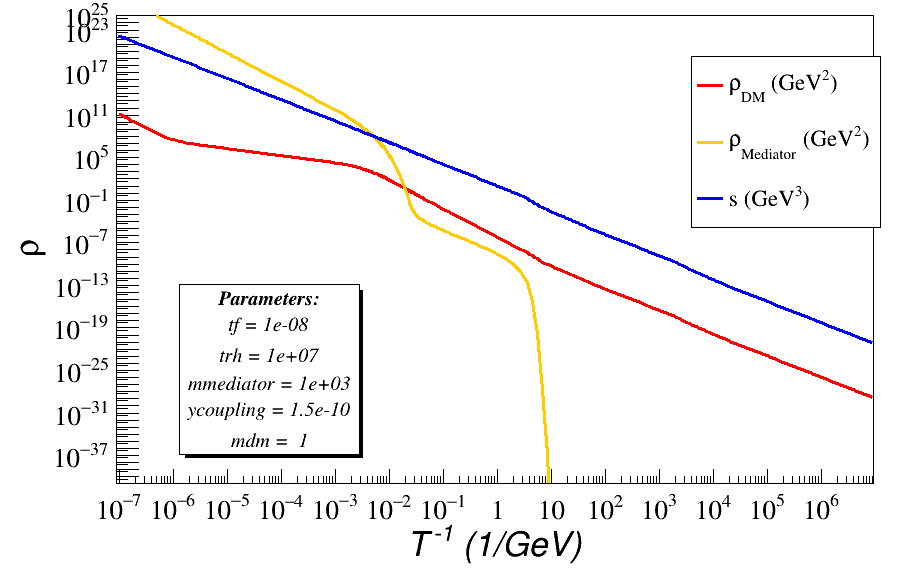
\includegraphics[width=0.5\linewidth,clip]{test.png}
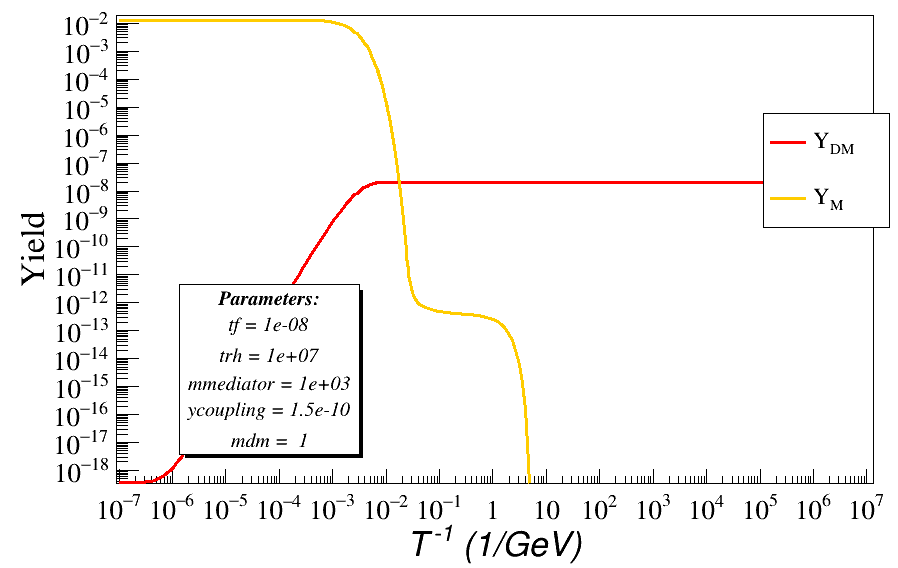
\includegraphics[width=0.5\linewidth,clip]{yield.png}
\caption{{\it Left}: Evolution of the mediator and DM energy densities ($\rho_M$ and $\rho_{DM}$)
as a function of the inverse of temperature. The evolution of the entropy density ($s$) is also shown.
{\it Right:} Evolution of the mediator and DM yields as a function of the inverse of temperature.
The parameters shown refer to the simplified FIMP scenario described in Sec.\ref{sec:simp}.
 \label{fig:solution1}}
\end{figure}

\subsection{Analytical Solution} \label{sec:analytic}

In order to analytically solve Eq.(\ref{eq:nDM}), we make the following assumptions:
\bi
\item a  weakly coupled DM, so $n_S/\bar{n}_S \ll 1$ and  $\langle \sigma v \rangle \bar{n}_S^2 \simeq 0$;
\item a strongly coupled mediator, so $n_M = \bar{n}_M$ and $\gamma_M$ is given by Eq.(\ref{eq:gamma});
\item a radiation dominated universe, so $H=\sqrt{\frac{8 \pi^3}{90}\frac{g_*(T) T^4}{M_P^2}}$;
\item entropy conservation ($\dot{S} = 0$).
\ei

Under the above assumtions Eq.(\ref{eq:nDM}) simplifies to:
\be
\Drv{n_{S}}{t} + 3H n_S  \simeq  \frac{\Gamma_M}{\gamma_M}  n_M
\ee
which, together with entropy conservation, leads to the following equation for the yield ($Y_S = n_S/s$):

\be
\Drv{Y_{S}}{t}  \simeq  \frac{\Gamma_M}{\gamma_M}  Y_M
\ee

Using $d/dt = -H T d/dT$, we have:

\be
\Drv{Y_S}{T} = -\frac{\Gamma_M}{\gamma_M}  \frac{Y_M}{H T} \Rightarrow Y_S = \Gamma_M   \int^{T_{RH}}_{0} \frac{1}{\gamma_M} \frac{Y_M}{H T} dT
\ee

Finally, using the assumption that the mediator is always in thermal equilibrium:

\be
\frac{Y_M}{\gamma_M} = \frac{1}{s} \frac{m_M^2 T}{2\pi^2} K_1\left(m_M/T\right)
\ee
and defining $x=m_M/T$, we obtain:

\be
Y_S = \left(\frac{45}{4 \pi^4} \frac{M_P}{1.66}\right)  g_M \frac{\Gamma_M}{m_M^2}   \int_{m_M/T_{RH}}^{\infty}  \frac{K_1(x) x^3}{\sqrt{g_*(m_M/x)} g_*^{S}(m_M/x)} dx
\ee
where we used $s = \frac{2 \pi^2}{45} g_*^{S}(T) T^3$.

If we further assume that $g_*(m_M/x), g_*^{S}(m_M/x) \simeq g_*(m_M), g_*^{S}(m_M)$ and $T_{RH} \gg m_M$, the integral
can be evaluated, giving:
\be
Y_S = \left(\frac{135}{8 \pi^3} \frac{M_P}{1.66}\right)  g_M \frac{\Gamma_M}{m_M^2} \frac{4.71}{\sqrt{g_*(m_M)} g_*^{S}(m_M)}
\ee



\section{Simplified FIMP Scenario} \label{sec:simp}

If we define the $S$-$M$-SM coupling as:
\be
y S M P_{SM}
\ee
and assume the mediator has gauge couplings to the SM, we have:

\be
\Gamma_M  = \frac{y^2}{8 \pi} m_M, \; \langle \sigma v \rangle_M  \simeq \frac{\alpha}{m_M^2}, \; \langle \sigma v \rangle_S  \simeq \frac{y^4}{m_S^2}
\ee
and $f_x = 1/2$, where $f_x$ is the fraction of energy injected in the thermal bath coming from $M \to S + X$ decays, which
is valid for $m_M \gg m_S$.

With the above definitions we can numerically and analytically compute the relic abundance
of DM, following the procedures described in Secs.\ref{sec:num} and \ref{sec:analytic}.
In Fig.\ref{fig:fig2}  we show the relic abundance as a function of $y$ for both the
analytic and the numerical solution.







\end{document}
